\documentclass[a4paper,10pt]{article}
\usepackage[utf8]{inputenc}
\usepackage[spanish,es-tabla]{babel}

\usepackage[a4paper,headheight=43pt,
            scale={0.8,0.8},hoffset=0.5cm,voffset=1cm]{geometry}

\usepackage{verbatim}

% paquetes matemáticos básicos
\usepackage{amsmath}
\usepackage{amsfonts}
\usepackage{amssymb}
\usepackage{xfrac}
\usepackage{siunitx}


% tikz
\usepackage{tikz}

% Código
\usepackage{listings}

\definecolor{codegreen}{rgb}{0,0.6,0}
\definecolor{codegray}{rgb}{0.5,0.5,0.5}
\definecolor{codepurple}{rgb}{0.58,0,0.82}
\definecolor{backcolour}{rgb}{0.95,0.95,0.92}

\lstdefinestyle{mystyle}{
    backgroundcolor=\color{backcolour},   
    commentstyle=\color{codegreen},
    keywordstyle=\color{magenta},
    numberstyle=\tiny\color{codegray},
    stringstyle=\color{codepurple},
    basicstyle=\ttfamily\footnotesize,
    breakatwhitespace=false,         
    breaklines=true,                 
    captionpos=b,                    
    keepspaces=true,                 
    numbers=left,                    
    numbersep=5pt,                  
    showspaces=false,                
    showstringspaces=false,
    showtabs=false,                  
    tabsize=2
}

\lstset{style=mystyle}

% gráficos
\usepackage{graphicx}
\usepackage{float}
\usepackage{caption}
\usepackage{subfig}
\usepackage{listings}
\captionsetup[table]{font={small,sc},labelfont={small,sc}}

\usepackage[subrefformat=parens]{subcaption} % para colocar subfiguras con sus
                                             % respectivas referencias,
                                             % subrefformat es para que ponga
                                             % parentesis en las subref

\usepackage{appendix}
\usepackage[output-decimal-marker={,},per-mode=symbol-or-fraction,retain-unity-mantissa=true,detect-all,range-phrase={ -- },list-final-separator={ y }]{siunitx}
%output-decimal-marker define el separador decimal que se imprime
%per-mode define la forma que se utiliza para mostrar las unidades del denominador, en este caso elije segun el modo matematico que usa
%retain-unity-mantissa define si muestra o no la mantisa cuando es 1
%detect-all detecta la fuente que corresponde al entorno donde se colocan las unidades
%range-phrase define la palabra para los rangos de numeros
%list-final-separator define la palabra final de las listas

% paquete para insertar hipervínculos (sólo para el encabezado)
\usepackage[colorlinks=true,urlcolor=blue,
            linkcolor=black,linktoc=none,citecolor=black]{hyperref}

\usepackage[twoside]{fancyhdr}		% formato de página
\usepackage{lastpage}
% Configuración del encabezado y pie de página
\fancyhf{} % Limpia todos los campos de encabezado y pie de página
%\fancyhead[L]{\textbf{TB070 Dispositivos Semiconductores}}
\fancyfoot{} % Limpia el pie de página para personalizarlo a continuación

\fancyfoot[LE,RO]{\thepage/\pageref{LastPage}}
\fancyfoot[LE,RO]{\thepage/\pageref{LastPage}}

%*** redefino el comportamiento de los apendices
\renewcommand{\appendixname}{Apéndices}
\renewcommand{\appendixtocname}{Apéndices}
\renewcommand{\appendixpagename}{Apéndices}
%\renewcommand{\tablename}{Tabla}
%\renewcommand\spanishtablename{Tabla}
%\renewcommand{\figurename}{Figura}
%***
\pagestyle{fancy}

\usepackage[dvipsnames]{xcolor}
%\usepackage{todonotes}		% ToDo List
\usepackage{hyperref}		% formato de página
\usepackage{tcolorbox}

\DeclareSIUnit\angstrom{\text {Å}}

% \newif\ifturnotarde
% %     \turnotardetrue
% \newif\ifturnonoche
%     \turnonochetrue

\begin{document}

% Defino el formato del encabezado
%\pagestyle{fancy}
% \lhead{\includegraphics[width=0.3\textwidth]{lhead}}
% \chead{
%   {\scshape Dispositivos Semiconductores}\\
%   {\footnotesize 1\textsuperscript{er} cuatrimestre de 2023}
% }
%\rhead{\includegraphics[width=0.1\textwidth]{rhead}}
\lfoot{}
\cfoot{\thepage}
\rfoot{}
\begin{titlepage}

\thispagestyle{empty}

\begin{center}
    
\includegraphics[scale=0.3]{fiuba.pdf}\\
    \large{\textsc{Universidad de Buenos Aires}}\\
    \large{\textsc{Facultad de Ingeniería}}\\
    % Modificar año y cuatrimestre
    \small{Año 2026 - 1\textsuperscript{er} cuatrimestre}
\end{center}

\vfill
% Redefino la numeracion de las subsecciones
\renewcommand{\thesubsection}{\arabic{subsection}}

\begin{center}
	{\LARGE \underline{\textbf{Taller de Automatización y Control (TA135)}}}\\[0.5cm]
	{\LARGE \textbf{Trabajo Práctico 1:
}}\\[0.5cm] 
    {\LARGE \textbf{Introducción al control digital
}}\\[0.5cm]
\end{center}

\begin{table}[H]
    \centering
    \begin{tabular}{|l|l|l|}
    \hline
    \multicolumn{3}{|c|}{\textbf{Integrantes Grupo N° 2}}    \\ \hline
    \multicolumn{1}{|l|}{Nombre y apellido} & Padrón & Correo \\ \hline
    \multicolumn{1}{|l|}{Juan Ignacio Biancuzzo}    & 106005 & jbiancuzzo@fi.uba.ar \\ \hline
    \multicolumn{1}{|l|}{Rocio Nicole Heredia Piñon}   & 107621 & rherediap@fi.uba.ar \\ \hline
    \end{tabular}
\end{table}

\vfill

\end{titlepage}

\tableofcontents
\newpage

\section{Limitaciones de los sensores}
\begin{itemize}
    \item Indicar la mínima resolución en la lectura del potenciómetro en volts y en grados. Calcular y/o estimar el tiempo requerido para realizar una medición.
    
    \item Indicar la mínima resolución en la lectura del sensor de distancia en segundos y en metros (u otra unidad según lo considere adecuado). Calcular y/o estimar el tiempo requerido para realizar una medición.

    \item Indicar la mínima resolución en la estimación del ángulo de la IMU en grados, considerando un estado estático (es decir, con la IMU en un ángulo fijo sin moverse). Calcular y/o estimar el tiempo requerido para realizar una medición.
\end{itemize}

\subsection{Potenciómetro}
Se conecta el potenciómetro al Arduino y se mide la tensión analógica del divisor resistivo, que tomará valores entre \SI{0}{\volt} y \SI{5}{\volt}. Como el ADC es de 10 bits, los valores posibles son de 0 a 1023. La resolución de la lectura del potenciómetro en volts, es decir, el menor cambio de tensión que el Arduino puede distinguir al leer la entrada, se puede calcular directamente como $\frac{\SI{5}{\volt}}{1024} = \SI{4.88}{\milli\volt}$. También se puede, a partir del valor analógico medido del potenciómetro, indicar el ángulo de posicionamiento de la perilla. Este tiene un rango de \SI{0}{\degree} a \SI{270}{\degree}, y su resolución queda determinada como $\frac{\SI{270}{\degree}}{1024} = \SI{0.26}{\degree}$.

Además, se pudo estimar el tiempo requerido para realizar la medición que resultó en \SI{105}{\micro\second}, y al usar la función \lstinline[language=c]{micros()} se espera tener una variación mínima de \SI{1}{\micro\second}.

\subsection{Sensor de distancia}

La mínima resolución en la lectura del sensor de distancia indica el mínimo intervalo de distancia que puede ser distinguido, la cual se extrajo de una datasheet \cite{sensor-disntacia} que fija la resolución en \SI{0.3}{\centi\meter}. Esto corresponde a aproximadamente \SI{8}{\micro\second} tomando la velocidad del sonido como \SI{340.29}{\meter/\second}. Es decir, que si el objeto se mueve una distancia menor a \SI{0.3}{\centi\meter}, el sensor no puede notar la diferencia y va a seguir leyendo lo mismo. El tiempo de ida y vuelta que mide el sensor, se refleja en el tiempo en el que el pulso en el pin Echo se mantiene en alto. Esto es lo que lee el Arduino, que lo puede hacer a través de funciones como \lstinline[language=c]{pulseIn()}. Leer el pin, compararlo con el valor esperado e incrementar el contador para pasar a la siguiente iteración toma $16$ ciclos de reloj. Entonces si la duración del pulso en alto es menor a \SI{1.33}{\micro\second} aproximadamente, el Arduino puede no llegar a leerlo. Como de todas formas el sensor de distancia en sí tiene una resolución menor, de \SI{8}{\micro\second}, esta termina siendo la resolución de toda la lectura del sensor de distancia. 

El tiempo requerido para la medición de distancia del sensor depende de la distancia del objeto de estudio. Mientras más lejos está, mayor será el tiempo de vuelo y por ende el tiempo de medición. A velocidad de sonido constante, se espera que el tiempo de medición varíe linealmente con la distancia. Se realiza la prueba en el Arduino y se realiza el gráfico de la figura \ref{fig:sensor_distancia}.

Se puede calcular la recta de regresión y observar el tiempo que requiere de medición una distancia que iguale el largo de la barra. El tiempo de medición variaría aproximadamente entre \SI{2449}{\micro\second} y \SI{4978}{\micro\second}, considerando distancias entre \SI{2}{\centi\meter}, que es la mínima en el rango de medición del sensor y \SI{45}{\centi\meter}, que es el largo de la barra.

\begin{figure}[H]
    \centering
    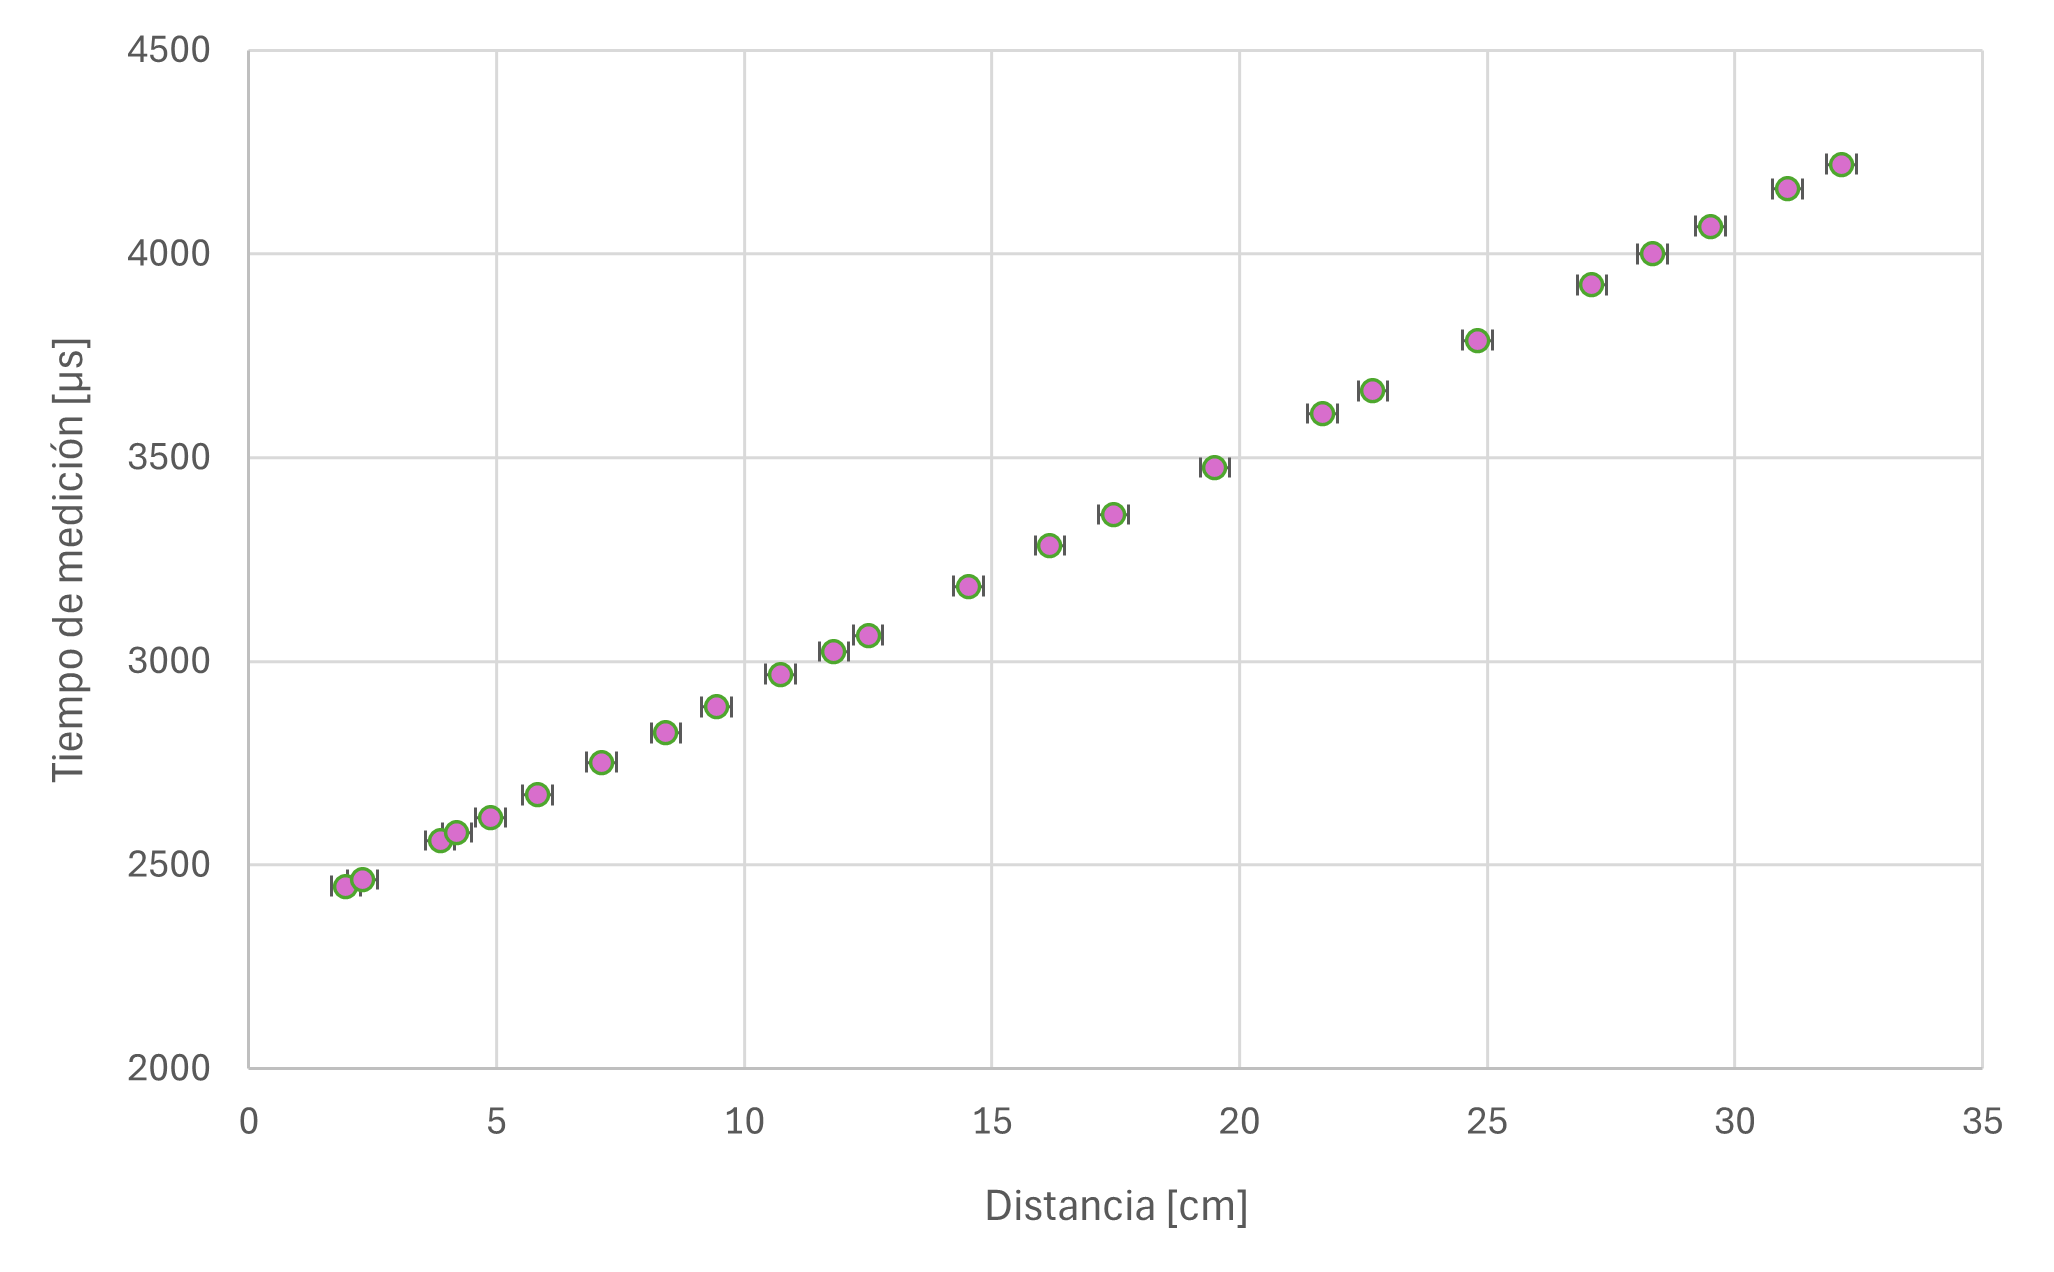
\includegraphics[width=0.8\linewidth]{imagenes/tiempo_sensor_distancia.png}
    \caption{Tiempo requerido para la medición del sensor HC-SR04 en función de la distancia.}
    \label{fig:sensor_distancia}
\end{figure}


\subsection{IMU}
Ambos sensores tienen su propio ADC de \SI{16}{\bit}, que convierten la señal analógica generada internamente en un número digital, que luego lee el Arduino. Los valores que podrán tomar las mediciones varían de 0 a 65635, por lo que esto repartido en cada rango correspondiente define la resolución. Se puede observar el resultado de estos cálculos dependiendo del rango elegido en la tabla \ref{tab:resoluciones_imu}. 

\begin{table}[H]
    \centering
    \begin{tabular}{|c|c||c|c|}
        \hline
        Rango [\SI{}{\degree / \second}] & Resolución giroscopio [$10^{-3}~$\SI{}{\degree / \second}] & Rango [g \SI{}{\meter / \second^2}] & Resolución acelerometro [g \SI{}{\micro\meter / \second^2}] \\\hline
        \SI{\pm 250}{} & \SI{7.63}{} & \SI{\pm 2}{} & \SI{30.52}{} \\\hline
        \SI{\pm 500}{} & \SI{15.26}{} & \SI{\pm 4}{} & \SI{61.04}{} \\\hline
        \SI{\pm 1000}{} & \SI{30.52}{} & \SI{\pm 8}{} &  \SI{122.07}{} \\\hline
        \SI{\pm 2000}{} & \SI{61.04}{} & \SI{\pm 16}{} & \SI{244.14}{} \\\hline
    \end{tabular}
    \caption{Resoluciones de la IMU.}
    \label{tab:resoluciones_imu}
\end{table}

Se pudo estimar el tiempo requerido para realizar la medición utilizando la función \lstinline[language=c]{micros()} en Arduino. Este tiempo resultó ser, en promedio, de \SI{3075}{\micro\second}, con un mínimo de \SI{3036}{\micro\second} y máximo de \SI{3096}{\micro\second}. 

% en microsegundos
% promedio 3075
% mínimo 3036
% máximo 3096

\section{Limitaciones de los actuadores}
Considere que el servomotor se controla a una frecuencia de \SI{50}{\hertz}, controlado por Arduino.
\begin{itemize}
    \item Indicar la mínima precisión angular que puede comandarse al servomotor y a la barra. Para ello
considere cómo un pin de PWM de Arduino genera la señal PWM correspondiente.
    \item Calcular y/o estimar el tiempo requerido para mover el servo un diferencial de \SI{30}{\degree}.
    \item Indicar cuál sería la diferencia en los puntos anteriores si la frecuencia de control fuese de \SI{1}{\hertz}.
\end{itemize}

El servo recibe una señal PWM y traduce el ancho del pulso a cierto ángulo. Lo que hace el Arduino es poner el pin en alto e iniciar un contador. En la librería de Servo de Arduino, hay una conversión de microsegundos a ticks que toma los ciclos del reloj interno por microsegundo y lo divide por 8. En este caso, como la frecuencia del reloj es \SI{12}{\mega\hertz}, se tienen \SI{1.5}{} ticks por microsegundo, es decir, \SI{0.67}{\micro\second} por cuenta. Como no todo ancho de pulso es realizable, puede que dos comandos que se diferencien en menos de \SI{0.67}{\micro\second} se generen como dos pulsos de igual duración, y por ende dos ángulos iguales en el servo. El rango angular del servo va de \SI{-90}{\degree} a \SI{90}{\degree} y se comprobó que el rango en microsegundos va de \SI{544}{\micro\second} a \SI{2400}{\micro\second}. La resolución angular está dada por $\frac{\SI{180}{\degree}}{\SI{1856}{\micro\second}}\cdot \SI{0.67}{\micro\second} = \SI{0.065}{\degree}$. Este es el menor ángulo comandable del servo. 

Se realizaron pruebas con el servomotor montado en la planta y se comprobó que el rango angular máximo del servomotor para mover a la barra va de \SI{-42}{\degree} a \SI{66}{\degree}. Se utilizó la IMU para medir el ángulo de la barra ante distintos ángulos comandados del servomotor. Estos se muestran en el gráfico de la figura \ref{fig:angulos_barra_servo}, donde se incluye la recta de regresión que muestra la tendencia lineal que relaciona los ángulos de la barra y el servo. 

\begin{figure}[H]
    \centering
    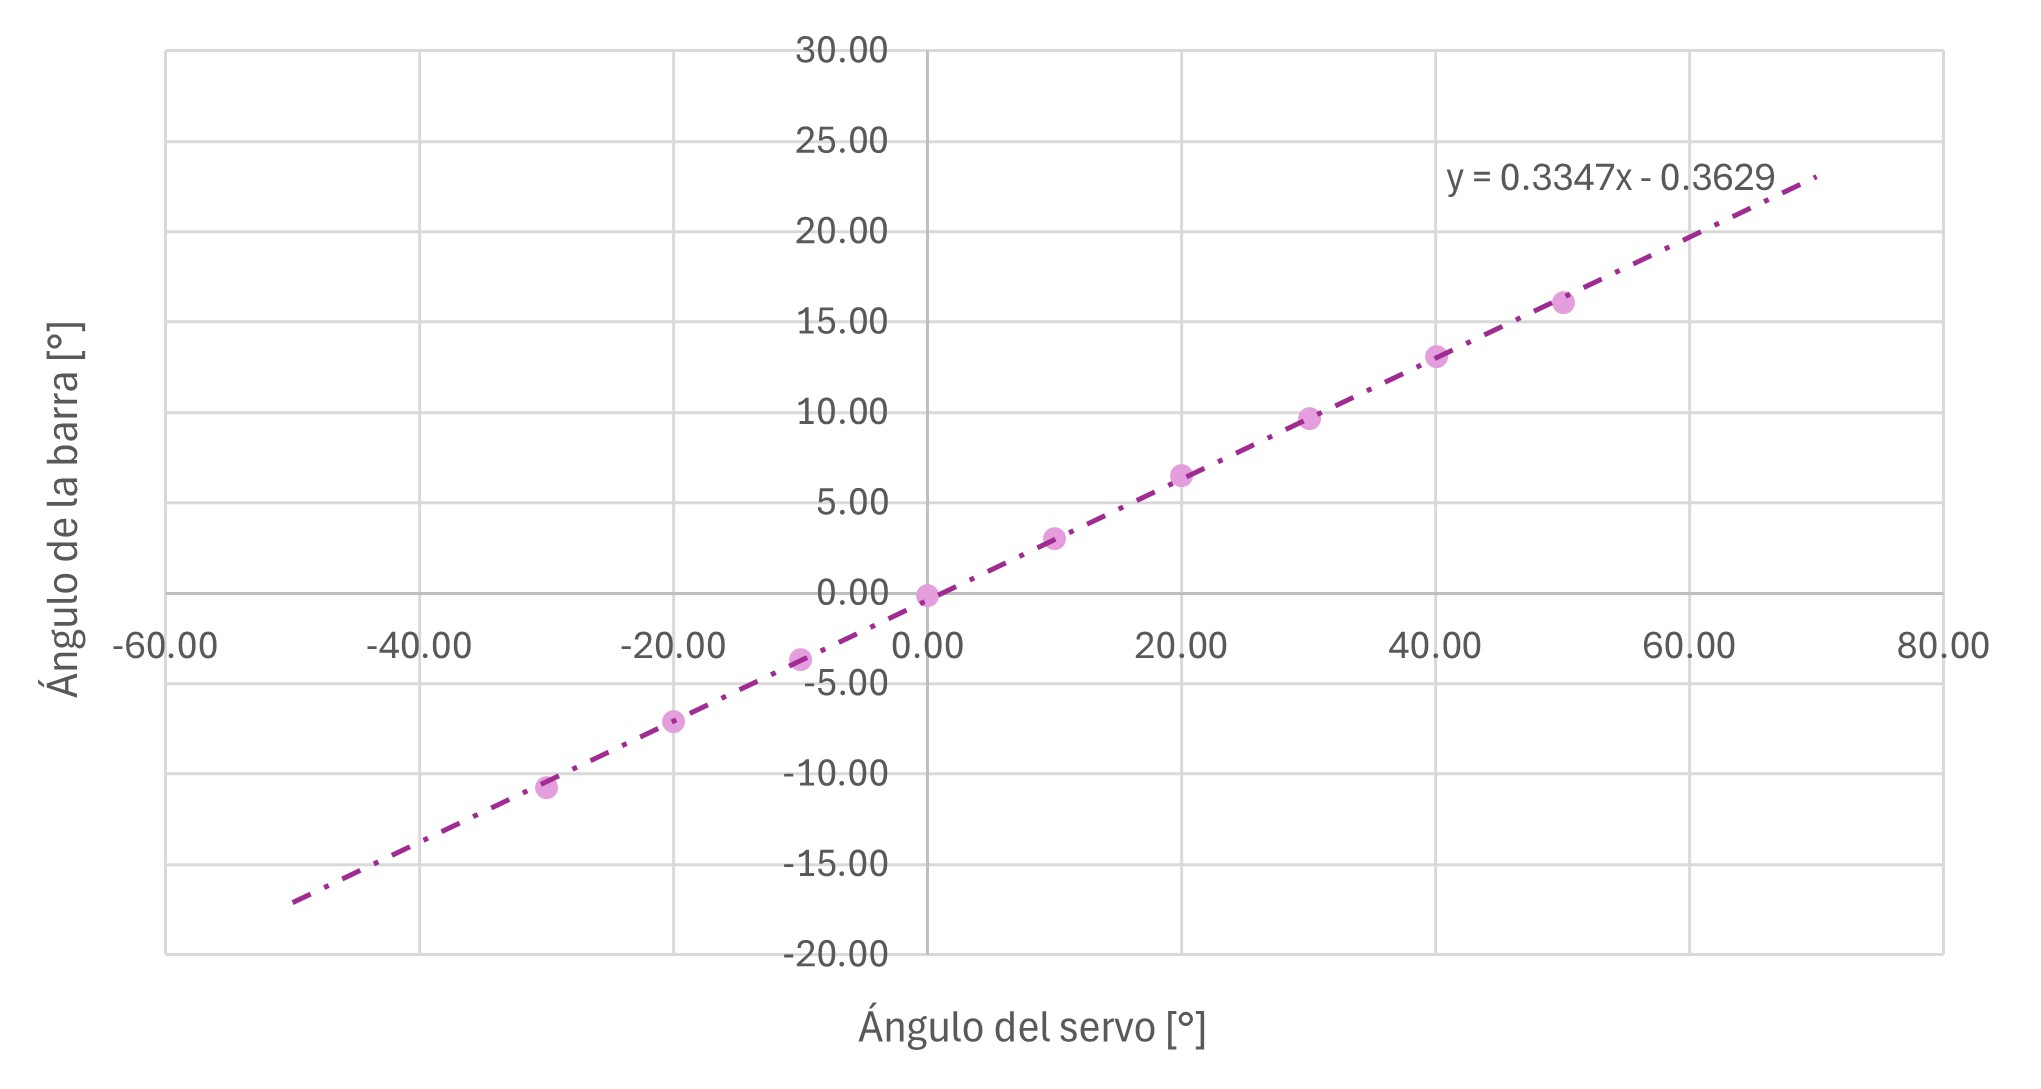
\includegraphics[width=0.8\linewidth]{imagenes/angulo_servo_barra.jpg}
    \caption{Mediciones de ángulos de la barra en función de los ángulos del servomotor. }
    \label{fig:angulos_barra_servo}
\end{figure}

En base a este comportamiento, si la mínima precisión angular comandable del servo es \SI{0.065}{\degree}, la de la barra será \SI{0.022}{\degree}.

Dentro de las pruebas que se realizaron, se chequeó el movimiento del servo ante diferenciales de ángulo pequeños y se comprobó que ante una variación menor a \SI{1}{\degree}, el servo no reaccionó. Por más que la resolución teórica es mucho mayor, en la práctica se concluyó que la resolución es de aproximadamente \SI{1}{\degree}, lo que se traduce a \SI{0.33}{\degree} de la barra. Esto no cambia con la frecuencia de control, y tampoco lo hace la mínima precisión angular comandable.

Se colocó el servo en \SI{0}{\degree}, y se comandó un diferencial de \SI{30}{\degree}. En la barra, se esperaría ver un ángulo de \SI{10.34}{\degree}, por lo que se toma el tiempo hasta que la IMU mide este ángulo de la barra. Este es el tiempo requerido para mover el servo un diferencial de \SI{30}{\degree}, y resultó ser igual a \SI{0.22}{\second} (prácticamente 10 veces el período de control). Esto cambia según la frecuencia de control.

En el programa desarrollado en Arduino, se realiza el sensado, procesamiento y actuación y se espera a llegar al período de control antes de ir a la siguiente iteración. Con una frecuencia de \SI{1}{\hertz} ese tiempo de espera es mayor. En la primera iteración, no se llega a medir el diferencial del ángulo (que ya se puede ver en el caso de \SI{50}{\hertz} que le toma 10 iteraciones). Pero luego espera hasta llegar a \SI{1}{\second}, que es tiempo en el que no se está haciendo nada. Y durante ese tiempo la barra ya llegó a la posición buscada, pero no se va a detectar hasta que termine el tiempo de espera y se vaya a la siguiente iteración. De esta forma, es esperable que el tiempo de medición crezca al disminuir la frecuencia de control. En este caso, el tiempo medido fue de \SI{1.003}{\second}. Para lograr esta medición, se tuvo que cambiar el $\alpha$ del filtro complementario, y darle más peso a la medición del ángulo del acelerómetro en comparación al giroscopio, porque con un $\Delta t$ tan grande, la medición acumuló mucho error. 

% HAS SIDO COMENTADO
\begin{comment}
    como el rango del servo va de 1ms para -90 a 2ms para 90, tenemos 1ms de rango completo, y nuestra función manda microsegundos, entonces tenemos 180/1000 = 0.18 grados de resolución.
Esto es asumiendo que el servo puede totalmente girar esa cantidad de grados
\end{comment}

% hacer transformacion de grados de la barra a grados del servo
% ver rango completo de la barra (nosotros podemos mandar más de 2ms y menos de 1ms para llegar a los mismos ) y ver microsegundos enviados para ver la resolución 
% Para los diferencia de 30 grados, usar la IMU para ver cuando llegamos a la posición correcta :) 

\section{Limitaciones de tareas adicionales}
\begin{itemize}
    \item Estime o mida el tiempo necesario para enviar $100$ floats ($4$ bytes cada uno) por el puerto serie de Arduino, a una velocidad de \SI{115200}{bps}. Indique cómo realizó el experimento. ¿Cúanto tiempo requerirá el envío de un único float, y porqué no se mide directamente?
\end{itemize}

Se calculó el tiempo necesario para enviar 100 floats. Para esto, se armó un array con los 400 bytes para pasárselo a \lstinline[language=c]{Serial.write()}, en este caso con caracteres. Luego, se espera a que se vacíe el buffer de transmisión usando 
\lstinline[language=c]{Serial.flush()} para poder medir correctamente el tiempo de transmisión.  
En cada iteración, se calcula este tiempo y se mantiene un registro del mínimo, el máximo, la cantidad de iteraciones realizadas y la suma acumulada, útil para obtener el promedio de las mediciones. De esta forma, se obtuvo un promedio de \SI{35493}{\micro\second}, con un mínimo de \SI{34012}{\micro\second} y con un máximo de \SI{35504}{\micro\second}.

% por 100 floats y las unidades de micro segundos
% 33988 tiempo promedio
% 28500 tiempo mínimo 
% 34008 tiempo máximo

El tiempo requerido para enviar un solo float se puede calcular directamente dividiendo los tiempos obtenidos para $100$ floats por $100$ y así alcanzando un promedio de \SI{354.93}{\micro\second}, con un mínimo de \SI{340.12}{\micro\second} y con un máximo de \SI{355.04}{\micro\second}. También se puede realizar el mismo proceso utilizado para los $100$ floats, enviando uno solo. Esta medición resultó en \SI{1658}{\micro\second} en promedio con un mínimo de \SI{1652}{\micro\second} y un máximo de \SI{1664}{\micro\second}. 


Para que sea comparable a la situación que se viene analizando, se puede pensar que en cada iteración del \lstinline{loop()} se envía un solo float, y se está midiendo el tiempo de $100$ iteraciones. En el momento de la transmisión existen dos causantes que atribuyen al tiempo medido, uno que se puede atribuir al proceso de empezar la comunicación y por lo tanto está dado por la cantidad de \lstinline{Serial.write()}, seguido de \lstinline{Serial.flush()}, y otro atribuible al procesamiento y envío de los datos útiles. Debe notarse, que el tiempo que es relevante para este análisis es el tiempo atribuible al envío de los datos útiles.

En la situación de análisis, se logra despreciar el tiempo atribuible al inicio de la comunicación ya que ocurre una vez. Por otro lado, en el caso de enviar un solo float, y medir $100$ iteraciones, este no se torna despreciable y por lo tanto no se logra medir el tiempo atribuible al envío de los datos útiles. 

% Se debe notar que el tiempo que se esta midiendo, y logramos obtener por medio del envío consecutivo de $100$ float, se puede  un overhead por los \SI{2}{\bit} (el start bit y el end bit, el default de arduino no incluye un bit de paridad y un solo end bit) extra a los bits útiles, ya que en los \SI{400}{\byte} se agrega este overhead.


% incluso se probo haciendo solo un llamado y el resuldo es el mismo, por lo que el over head del llamado de la función es completamente despreciables

% si el frame de uart es de 8 bits, el minimo deberia ser de 277 us que es aprox lo que vemos en el minimo, pero con un frame de 10 bits, que es en teoria lo que estamos mandando por el start bit y el end bit, entonces el minimo es de 347 us que es muy similar a nuestro máximo. Por lo tanto hay que ver que puede ser que sea el motivo, pero puede ser que tenga que ver con eso.
% la cuenta es (bitFrame x 4 x nFloats) / (115200)
% lo unico que mejora con un nFloats mayor es que si tuvieramos un ruido en la medicion pero tambien ya lo estamos promediando en general entonces ni idea 

% por 1 float y las unidades de micro segundos
% 337 tiempo promedio
% 332 tiempo mínimo
% 344 tiempo máximo

\section{Referencias}

\renewcommand{\section}[2]{}
\bibliographystyle{IEEEtran}
\bibliography{referencias.bib}

\end{document}
